\chapter{Interoperability Layer for Clinical Research Systems}
\label{sec:interoplayer}

% intro
Now that we have the architecture of our solution, this chapter covers the design and implementation of the first objective of our project: creating an interoperability layer for the clinical research systems i2b2 and tranSMART 17.1, that is exploitable by the front end Glowing Bear, and with the identity and access management handled by Keycloak.
Support for MedCo is covered in the next section.

% outline
We are first going over the detailed workflow of the system, showing the end-to-end processing of a query.
We are then detailing the design and implementation of the different parts solving the objective: the identity provider, the front-end, the API translation, and the processing in the back end systems.
Appendix~\ref{sec:docker} covers exhaustively the technical details of the Docker-based deployment of the system.


\section{Detailed Workflow}
\label{sec:interoplayer-wf}

\begin{figure}[ht]
    \centering
    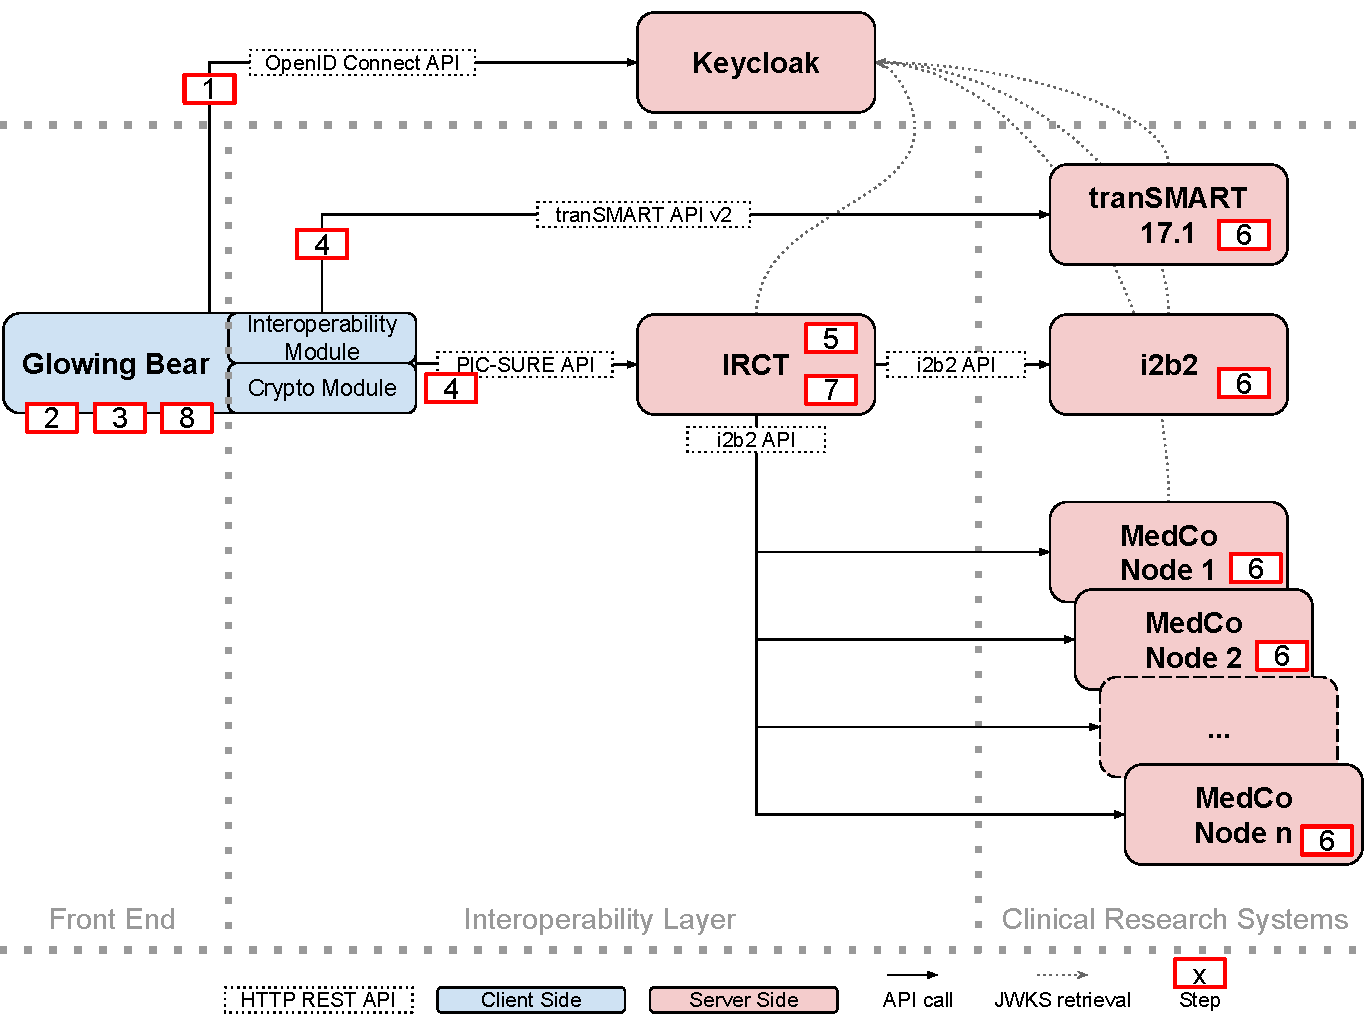
\includegraphics[width=1\textwidth]{figures/sys_diagram_full_with_steps.pdf}
    \caption{Full System Diagram, with execution steps}
    \label{fig:sys-diagram-full-steps}
\end{figure}

This section gives an overview of the full workflow of our system when constructing and executing a query.
Some steps are specific to \textit{tranSMART} 17.1 or \textit{PIC-SURE}.
The step numbering refers to figure~\ref{fig:sys-diagram-full-steps}.

\begin{enumerate}
\item \label{enum:wf-interop-login}\textbf{User Login}:
The user accesses Glowing Bear through its web browser, which redirects it to the Keycloak login page.
The user submits her credentials to Keycloak, which upon success redirects the user to Glowing Bear, giving at the same time the JSON Web Token (JWT)~\cite{rfc:jwt}, containing authentication and authorization information.
The user is thus logged in in the system.

\item \label{enum:wf-interop-init} \textbf{Glowing Bear Initialization}:
Glowing Bear reads from its configuration which type of back end it should use.
The tree of query terms is loaded, either entirely (\textit{tranSMART}) or only the root nodes (\textit{PIC-SURE}).
In the \textit{PIC-SURE} case, Glowing Bear fetches the definitions of the data sources set up on IRCT.

\item \textbf{Query Construction}:
The user browses the tree of query terms and uses them to construct a query corresponding to a patient set.
When adding a term into the query panel, Glowing Bear might, according to its type, make a background request to fetch the term metadata, which is the case for example for categorical or numerical terms.
The user then optionally sets value(s) to the query term.

\item \textbf{Query Submission}:
Upon user request (or automatically according to the configuration), Glowing Bear submits the query to the back end.

\item \textbf{Query Translation} \textit{PIC-SURE only}: IRCT uses the appropriate data source interface to perform the translation into the native i2b2 API of the query, and submits it to i2b2.

\item \textbf{Query Processing}: the submitted query, either directly from Glowing Bear for tranSMART or through IRCT for i2b2, is processed by the platform. 
The result is sent back to the requester.

\item \textbf{Result Storage} \textit{PIC-SURE only}: IRCT stores the result in its database, and sets the query as being successful.

\item \textbf{Result Display}: the result is displayed to the user in Glowing Bear.
Given the asynchronous nature of IRCT when processing queries, Glowing Bear periodically (every second) fetches the status of a \textit{PIC-SURE} query, and only after fetches its result.

\end{enumerate}


\section{Identity and Access Management}
\label{sec:interoplayer-idp}

% outline
This section first exposes how the authentication (identity) and authorization (access) are handled in our system with OpenID Connect and Keycloak, and then the steps taken to achieve this implementation.

\subsection{Authentication}

% overview
Authentication management is about verifying the identity of the user trying to access data.
With OpenID Connect, the authentication of the user is made by the identity provider, here Keycloak.
Keycloak can authenticate users in a number of ways: classic credentials (user and password) stored in its database, against external directories like LDAP, delegating to external OAuth2 or OIDC providers, and more.
Two-factors authentication using One-Time Password (OTP)~\cite{rayes2011one}, time (TOTP) or counter (HOTP) based, is also available.
This configuration, which can be specific to the client systems, is the responsibility of the administrator. 

% login process / authentication
When loaded, Glowing Bear checks for the presence and validity of the JWT. 
If not valid the user is redirected to the login page of Keycloak. 
In this redirection several parameters are passed:

\begin{itemize}
    \item the client identifier (\verb|client_id|): identify for which client system the authentication is made for.
    Here the client systems are set to be the clinical research systems, as they are the ones that enforce control over who can access their data. For example if Glowing Bear is set to use an i2b2 instance through PIC-SURE, the client could be \verb|i2b2-instance-1|.
    \item the redirection URL (\verb|redirect_uri|): the URL to which Keycloak should redirect the user after login, here it is set to be the URL of Glowing Bear.
    \item the type of token requested (\verb|response_type|): the type of token requested, this defines which flow is used (see below). We use \verb|code| in order to use the \emph{authorization code} flow.
\end{itemize}

% flow / after login / values login OK
Once the authentication is successful, several behaviors (called flows) can happen between the authentication of the user and the verification of the token at the client system.
We focus on the behavior we use, the \emph{authorization code} flow.
Keycloak redirects the user back to Glowing Bear, giving the authorization code at the same time.
Glowing Bear then exchanges this authorization code for the following tokens in the background:

\begin{itemize}
    \item an \emph{access token}: this is the signed JWT that contains the identity and authorizations of the user. It is sent along with the HTTP requests made to the back end systems. An example of a JWT is provided in section~\ref{sec:bg-oidc}.
    \item a \emph{refresh token}: when the access token expires, Glowing Bear uses the refresh token to request a new one. This can be done in the background without user interaction as long as the login session with Keycloak is still valid.
\end{itemize}

% using the tokens from gb
Glowing Bear embeds the access token into every HTTP request that needs to be authenticated.
It is done by adding the following HTTP header, which is specified by~\cite{rfc:bearertoken}:
\begin{verbatim}
    Authorization : Bearer <token>
\end{verbatim}

% validating tokens from the back end
Validating an access token in the JWT format requires several checks, performed in the back end systems~\cite{rfc:oidc}.
The prerequisite to those checks is that the back end system should fetch from Keycloak its public signing keys, which are made available in the JSON Web Key Set format (JWKS)~\cite{rfc:jwk}.
The checks are:

\begin{itemize}
    \item the issuer of the token should be the expected Keycloak instance (\verb|iss| field)
    \item the client identifier should be the identifier of the expected back end system (\verb|aud| field)
    \item the token must not be expired (\verb|exp| field)
    \item the signature of the token should be valid (\verb|RS256| signature: SHA-256 with RSA signature, in JSON Web Signature (JWS)~\cite{rfc:jws} format)
\end{itemize}

Using this authentication mechanism, the back end systems have a stateless authentication that needs only Keycloak's URL, the client identifier and the token.

\subsection{Authorization}

% overview
Authorization management is about restricting access to data depending on the access level of the user.
With OIDC, the authorizations of a user are embedded as a \emph{claim} into the JWT by the identity provider.
While the authorizations are set at the identity provider, their enforcement are the responsibility of the client system, in this case tranSMART. 
Note that i2b2 and IRCT do not use the authorization capabilities of OIDC, only its authentication mechanism.

% authorization encoding
The standard does not specify a format for encoding authorizations, it is left at the client system's discretion.
As Keycloak has its own format of authorization encoding, it also provides the ability to map authorizations to a specific format according to the client.
It is thus the responsibility of the administrator doing the deployment to make these two formats match by using the mapping capabilities of Keycloak.


\subsection{Implementation}

\subsubsection{Glowing Bear}

% add oidc support + http interceptor
Glowing Bear originally makes use of the client side of the OAuth2~\cite{rfc:oauth2} protocol for authorization with tranSMART. 
We thus modify it to use the OpenID Connect protocol.
To embed the JWT into the HTTP requests an interceptor is implemented. 
It intercepts all the requests made by Glowing Bear, examines them, and adds in the headers the token if it is needed.
This way, the requests can be authenticated by the receiving back end.

\subsubsection{IRCT}

% RS256 implementation
In its original implementation IRCT supports only JWT with a \verb|HS256| signature, i.e. a shared-secret based signature. 
Because Keycloak does not support this type of signature, and because the standard recommends to use \verb|RS256| signature~\cite{rfc:oidc}, we modify the IRCT implementation to do so. 
The support of \verb|RS256| signatures is added alongside \verb|HS256|, which instead of the shared secret needs as input the public signing keys of Keycloak.
The retrieval of those in the JWKS format is thus implemented, from a URL specified in the configuration.
The verification of the token is voluntarily incomplete: checking for the issuer and the client identifier is left as the responsibility of the back end system queried by IRCT.

\subsubsection{i2b2}

% oidc compat and parameters i2b2
i2b2 initially supports authentication with its own user management mechanism or through LDAP or NTLM directories.
We take advantage of the i2b2 Project Management (PM) cell ability to specify in the database the authentication mechanism to implement the support of OpenID Connect.
This allows users authenticated with OIDC to cohabit with users authenticated with the traditional i2b2 way.
This is done through the i2b2 PM parameters (as specified section~\ref{sec:bg-i2b2}), which can be applied either at user, cell or project level. 
They are the following:

\begin{itemize}
    \item token issuer (Keycloak instance URL)
    \item signing public keys URL (JWKS)
    \item client identifier
    \item field name in the JWT of the user's username
\end{itemize}

This last field is needed to ensure that the user account in the i2b2 database matches the user specified in the token, in order to enforce the authorizations.
Because there is no such thing as a standard username field, it needs to be specified by the configuration.

% how token is sent
The token is passed through the \verb|password| field of the i2b2 XML API.
This approach is not among the recommended ones, but it does not go against the OpenID Connect standard, and it simplifies greatly the implementation.
